\wde{Graphical Models}{
    Aid readability and understanding of a machine learning model.
}

\we{Confounder / Mediator}{
    % draw a graph where U -> Smoking and U-> Stroke and Smoking -> HIV and Smoking -> Stroke and HIV -> Stroke and Age -> HIV and Age -> Stroke and Age -> Smoking
      Let $U$ be the unknown or unmeasured variable. $S$ be smoking, $St$ be stroke, $H$ be HIV and $A$ be age.
      \begin{center}
      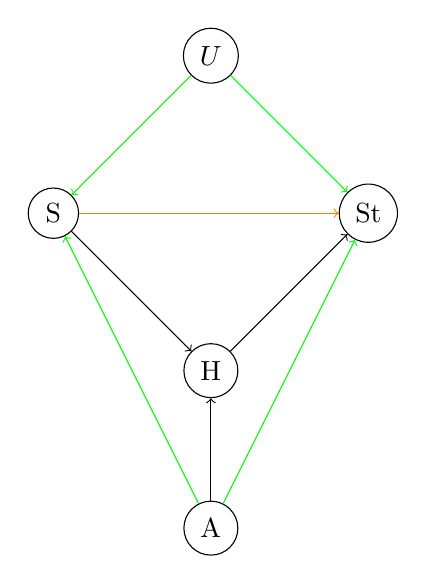
\begin{tikzpicture}
      % nodes
    %    \node[obs] (x) {$x$};%
    %    \node[latent,above=of x,xshift=-1cm,fill] (y) {$y$}; %
    %    \node[latent,above=of x,xshift=1cm] (z) {$z$}; %
    %    \draw (0,1.69) circle(.36cm);
    %   % plate
    %    \plate [inner sep=.25cm,yshift=.2cm] {plate1} {(x)(y)(z)} {$N$}; %
    %   % edges
    %    \edge {y,z} {x} 
        \node[draw, circle] (U) at (3,0) {$U$};
        \node[draw, circle] (smoke) at (1,-2) {S};
        \node[draw, circle] (stroke) at (5,-2) {St};
        \node[draw, circle] (hiv) at (3,-4) {H};
        \node[draw, circle] (age) at (3,-6) {A};
        \draw[draw=green,->] (U) -- (smoke);
        \draw[draw=green,->] (U) -- (stroke);
        \draw[->] (smoke) -- (hiv);
        \draw[draw=orange,->] (smoke) -- (stroke);
        \draw[->] (hiv) -- (stroke);
        \draw[->] (age) -- (hiv);
        \draw[draw=green,->] (age) -- (stroke);
        \draw[draw=green,->] (age) -- (smoke);
      \end{tikzpicture}
      \end{center}
      If we were investigating the relationship between smoking and stroke, then $U$ and $A$ are confounders i.e.
      age is a predictor for strokes. 
      $H$ is a mediator i.e. HIV has a casual effect on strokes.
}


\wde{(directed) Graph Representation}{
    A directed graph is a set of nodes connected by edges.
    Each vertex is a random variable and each edge represents a direct dependency.
    It is directed and acyclic (DAG).
    A distribution factorises according to the graph if 
    $$
    p(x_1, \ldots, x_n) = \prod_{i=1}^n p(x_i | \text{parents}(x_i))
    $$
}
\wde{Graph structures}{
    \begin{itemize}
    \item Chain $x \perp z | y$
    \begin{center}
        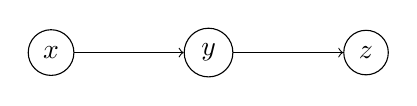
\begin{tikzpicture}
            \node[draw, circle] (x) at (0,0) {$x$};
            \node[draw, circle] (y) at (2,0) {$y$};
            \node[draw, circle] (z) at (4,0) {$z$};
            \draw[->] (x) -- (y);
            \draw[->] (y) -- (z);
        \end{tikzpicture}
    \end{center}
    \item Common cause $x \perp z | y$
    \begin{center}
        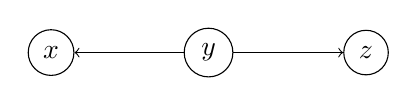
\begin{tikzpicture}
            \node[draw, circle] (x) at (0,0) {$x$};
            \node[draw, circle] (y) at (2,0) {$y$};
            \node[draw, circle] (z) at (4,0) {$z$};
            \draw[->] (y) -- (x);
            \draw[->] (y) -- (z);
        \end{tikzpicture}
    \end{center}
    \item v-structure $x \perp z$ but $x \not\perp z | y$
    \begin{center}
        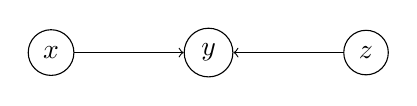
\begin{tikzpicture}
            \node[draw, circle] (x) at (0,0) {$x$};
            \node[draw, circle] (y) at (2,0) {$y$};
            \node[draw, circle] (z) at (4,0) {$z$};
            \draw[->] (x) -- (y);
            \draw[->] (z) -- (y);
        \end{tikzpicture}
    \end{center}
    \end{itemize}
}